% Options for packages loaded elsewhere
\PassOptionsToPackage{unicode}{hyperref}
\PassOptionsToPackage{hyphens}{url}
%
\documentclass[
]{article}
\usepackage{lmodern}
\usepackage{amssymb,amsmath}
\usepackage{ifxetex,ifluatex}
\ifnum 0\ifxetex 1\fi\ifluatex 1\fi=0 % if pdftex
  \usepackage[T1]{fontenc}
  \usepackage[utf8]{inputenc}
  \usepackage{textcomp} % provide euro and other symbols
\else % if luatex or xetex
  \usepackage{unicode-math}
  \defaultfontfeatures{Scale=MatchLowercase}
  \defaultfontfeatures[\rmfamily]{Ligatures=TeX,Scale=1}
\fi
% Use upquote if available, for straight quotes in verbatim environments
\IfFileExists{upquote.sty}{\usepackage{upquote}}{}
\IfFileExists{microtype.sty}{% use microtype if available
  \usepackage[]{microtype}
  \UseMicrotypeSet[protrusion]{basicmath} % disable protrusion for tt fonts
}{}
\makeatletter
\@ifundefined{KOMAClassName}{% if non-KOMA class
  \IfFileExists{parskip.sty}{%
    \usepackage{parskip}
  }{% else
    \setlength{\parindent}{0pt}
    \setlength{\parskip}{6pt plus 2pt minus 1pt}}
}{% if KOMA class
  \KOMAoptions{parskip=half}}
\makeatother
\usepackage{xcolor}
\IfFileExists{xurl.sty}{\usepackage{xurl}}{} % add URL line breaks if available
\IfFileExists{bookmark.sty}{\usepackage{bookmark}}{\usepackage{hyperref}}
\hypersetup{
  hidelinks,
  pdfcreator={LaTeX via pandoc}}
\urlstyle{same} % disable monospaced font for URLs
\usepackage[margin=1in]{geometry}
\usepackage{color}
\usepackage{fancyvrb}
\newcommand{\VerbBar}{|}
\newcommand{\VERB}{\Verb[commandchars=\\\{\}]}
\DefineVerbatimEnvironment{Highlighting}{Verbatim}{commandchars=\\\{\}}
% Add ',fontsize=\small' for more characters per line
\usepackage{framed}
\definecolor{shadecolor}{RGB}{248,248,248}
\newenvironment{Shaded}{\begin{snugshade}}{\end{snugshade}}
\newcommand{\AlertTok}[1]{\textcolor[rgb]{0.94,0.16,0.16}{#1}}
\newcommand{\AnnotationTok}[1]{\textcolor[rgb]{0.56,0.35,0.01}{\textbf{\textit{#1}}}}
\newcommand{\AttributeTok}[1]{\textcolor[rgb]{0.77,0.63,0.00}{#1}}
\newcommand{\BaseNTok}[1]{\textcolor[rgb]{0.00,0.00,0.81}{#1}}
\newcommand{\BuiltInTok}[1]{#1}
\newcommand{\CharTok}[1]{\textcolor[rgb]{0.31,0.60,0.02}{#1}}
\newcommand{\CommentTok}[1]{\textcolor[rgb]{0.56,0.35,0.01}{\textit{#1}}}
\newcommand{\CommentVarTok}[1]{\textcolor[rgb]{0.56,0.35,0.01}{\textbf{\textit{#1}}}}
\newcommand{\ConstantTok}[1]{\textcolor[rgb]{0.00,0.00,0.00}{#1}}
\newcommand{\ControlFlowTok}[1]{\textcolor[rgb]{0.13,0.29,0.53}{\textbf{#1}}}
\newcommand{\DataTypeTok}[1]{\textcolor[rgb]{0.13,0.29,0.53}{#1}}
\newcommand{\DecValTok}[1]{\textcolor[rgb]{0.00,0.00,0.81}{#1}}
\newcommand{\DocumentationTok}[1]{\textcolor[rgb]{0.56,0.35,0.01}{\textbf{\textit{#1}}}}
\newcommand{\ErrorTok}[1]{\textcolor[rgb]{0.64,0.00,0.00}{\textbf{#1}}}
\newcommand{\ExtensionTok}[1]{#1}
\newcommand{\FloatTok}[1]{\textcolor[rgb]{0.00,0.00,0.81}{#1}}
\newcommand{\FunctionTok}[1]{\textcolor[rgb]{0.00,0.00,0.00}{#1}}
\newcommand{\ImportTok}[1]{#1}
\newcommand{\InformationTok}[1]{\textcolor[rgb]{0.56,0.35,0.01}{\textbf{\textit{#1}}}}
\newcommand{\KeywordTok}[1]{\textcolor[rgb]{0.13,0.29,0.53}{\textbf{#1}}}
\newcommand{\NormalTok}[1]{#1}
\newcommand{\OperatorTok}[1]{\textcolor[rgb]{0.81,0.36,0.00}{\textbf{#1}}}
\newcommand{\OtherTok}[1]{\textcolor[rgb]{0.56,0.35,0.01}{#1}}
\newcommand{\PreprocessorTok}[1]{\textcolor[rgb]{0.56,0.35,0.01}{\textit{#1}}}
\newcommand{\RegionMarkerTok}[1]{#1}
\newcommand{\SpecialCharTok}[1]{\textcolor[rgb]{0.00,0.00,0.00}{#1}}
\newcommand{\SpecialStringTok}[1]{\textcolor[rgb]{0.31,0.60,0.02}{#1}}
\newcommand{\StringTok}[1]{\textcolor[rgb]{0.31,0.60,0.02}{#1}}
\newcommand{\VariableTok}[1]{\textcolor[rgb]{0.00,0.00,0.00}{#1}}
\newcommand{\VerbatimStringTok}[1]{\textcolor[rgb]{0.31,0.60,0.02}{#1}}
\newcommand{\WarningTok}[1]{\textcolor[rgb]{0.56,0.35,0.01}{\textbf{\textit{#1}}}}
\usepackage{longtable,booktabs}
% Correct order of tables after \paragraph or \subparagraph
\usepackage{etoolbox}
\makeatletter
\patchcmd\longtable{\par}{\if@noskipsec\mbox{}\fi\par}{}{}
\makeatother
% Allow footnotes in longtable head/foot
\IfFileExists{footnotehyper.sty}{\usepackage{footnotehyper}}{\usepackage{footnote}}
\makesavenoteenv{longtable}
\usepackage{graphicx,grffile}
\makeatletter
\def\maxwidth{\ifdim\Gin@nat@width>\linewidth\linewidth\else\Gin@nat@width\fi}
\def\maxheight{\ifdim\Gin@nat@height>\textheight\textheight\else\Gin@nat@height\fi}
\makeatother
% Scale images if necessary, so that they will not overflow the page
% margins by default, and it is still possible to overwrite the defaults
% using explicit options in \includegraphics[width, height, ...]{}
\setkeys{Gin}{width=\maxwidth,height=\maxheight,keepaspectratio}
% Set default figure placement to htbp
\makeatletter
\def\fps@figure{htbp}
\makeatother
\setlength{\emergencystretch}{3em} % prevent overfull lines
\providecommand{\tightlist}{%
  \setlength{\itemsep}{0pt}\setlength{\parskip}{0pt}}
\setcounter{secnumdepth}{-\maxdimen} % remove section numbering

\author{}
\date{\vspace{-2.5em}}

\begin{document}

\hypertarget{musterloesung-aufgabe-4.2s-multiple-logistische-regression}{%
\subsection{Musterloesung Aufgabe 4.2S: multiple logistische
Regression}\label{musterloesung-aufgabe-4.2s-multiple-logistische-regression}}

\begin{center}\rule{0.5\linewidth}{0.5pt}\end{center}

\begin{quote}
\textbf{Lese-Empfehlung} Kapitel 6 von
\href{https://mgimond.github.io/Stats-in-R/Logistic.html}{Manny Gimond}
\end{quote}

\begin{quote}
\textbf{Lese-Empfehlung} Kapitel 4 von
\href{http://faculty.marshall.usc.edu/gareth-james/ISL/ISLR\%20Seventh\%20Printing.pdf}{Gareth
(2016)}
\end{quote}

\begin{quote}
Download \href{16_Statistik4/RFiles/solution_stat4.2s.R}{R-Skript}
\end{quote}

\begin{quote}
Download \href{16_Statistik4/RFiles/solution_stat4.2s.pdf}{PDF}
\end{quote}

\begin{center}\rule{0.5\linewidth}{0.5pt}\end{center}

\textbf{kommentierter Lösungsweg}

\begin{Shaded}
\begin{Highlighting}[]
\CommentTok{# Genereiert eine Dummyvariable: Fleisch 1, kein Fleisch 0}
\NormalTok{df <-}\StringTok{ }\NormalTok{nova_survey }\OperatorTok\StringTok{  }\CommentTok{# kopiert originaler Datensatz}
\StringTok{  }\KeywordTok{rename}\NormalTok{(}\DataTypeTok{umwelteinstellung =}\NormalTok{ tho_}\DecValTok{2}\NormalTok{) }\OperatorTok\StringTok{ }\CommentTok{# änderung name der variable}
\StringTok{  }\KeywordTok{mutate}\NormalTok{(}\DataTypeTok{umwelteinstellung =} \KeywordTok{case_when}\NormalTok{(umwelteinstellung }\OperatorTok{==}\StringTok{ }\DecValTok{4} \OperatorTok{~}\StringTok{ }\DecValTok{1}\NormalTok{,}
\NormalTok{                                       umwelteinstellung }\OperatorTok{==}\StringTok{ }\DecValTok{3} \OperatorTok{~}\StringTok{ }\DecValTok{1}\NormalTok{,}
\NormalTok{                                       umwelteinstellung }\OperatorTok{==}\StringTok{ }\DecValTok{2} \OperatorTok{~}\StringTok{ }\DecValTok{0}\NormalTok{, }
\NormalTok{                                       umwelteinstellung }\OperatorTok{==}\StringTok{ }\DecValTok{1} \OperatorTok{~}\StringTok{ }\DecValTok{0}\NormalTok{)) }\OperatorTok\StringTok{ }
\StringTok{  }\CommentTok{# lasse die kleine Gruppe mit x weg}
\StringTok{  }\NormalTok{dplyr}\OperatorTok{::}\KeywordTok{filter}\NormalTok{(}\OperatorTok{!}\KeywordTok{str_detect}\NormalTok{(}\DataTypeTok{string =} \StringTok{"x"}\NormalTok{, gender)) }\OperatorTok\StringTok{ }
\StringTok{  }\CommentTok{# lasse die kleine Gruppe "andere" weg}
\StringTok{  }\NormalTok{dplyr}\OperatorTok{::}\KeywordTok{filter}\NormalTok{(}\OperatorTok{!}\KeywordTok{str_detect}\NormalTok{(}\DataTypeTok{string =} \StringTok{"Andere"}\NormalTok{, member)) }\OperatorTok\StringTok{  }
\StringTok{  }\CommentTok{# wähle nur die relevanten variablen aus}
\StringTok{  }\NormalTok{dplyr}\OperatorTok{::}\KeywordTok{select}\NormalTok{(mensa, age_groups, gender, member, umwelteinstellung, meat) }

\CommentTok{# Schaut euch die Missings an in der Kriteriumsvariable "mensa"}
\KeywordTok{sum}\NormalTok{(}\KeywordTok{is.na}\NormalTok{(df}\OperatorTok{$}\NormalTok{mensa))}
\end{Highlighting}
\end{Shaded}

\begin{verbatim}
## [1] 0
\end{verbatim}

\begin{Shaded}
\begin{Highlighting}[]
\CommentTok{# schaut euch die Missings an in den Prädiktorvariablen "Alter", "Geschlecht", "Hochschulzugehörigkeit", "umwelteinstellung"}
\NormalTok{Amelia}\OperatorTok{::}\KeywordTok{missmap}\NormalTok{(df) }
\end{Highlighting}
\end{Shaded}

\begin{verbatim}
## Warning: Unknown or uninitialised column: `arguments`.

## Warning: Unknown or uninitialised column: `arguments`.
\end{verbatim}

\begin{verbatim}
## Warning: Unknown or uninitialised column: `imputations`.
\end{verbatim}

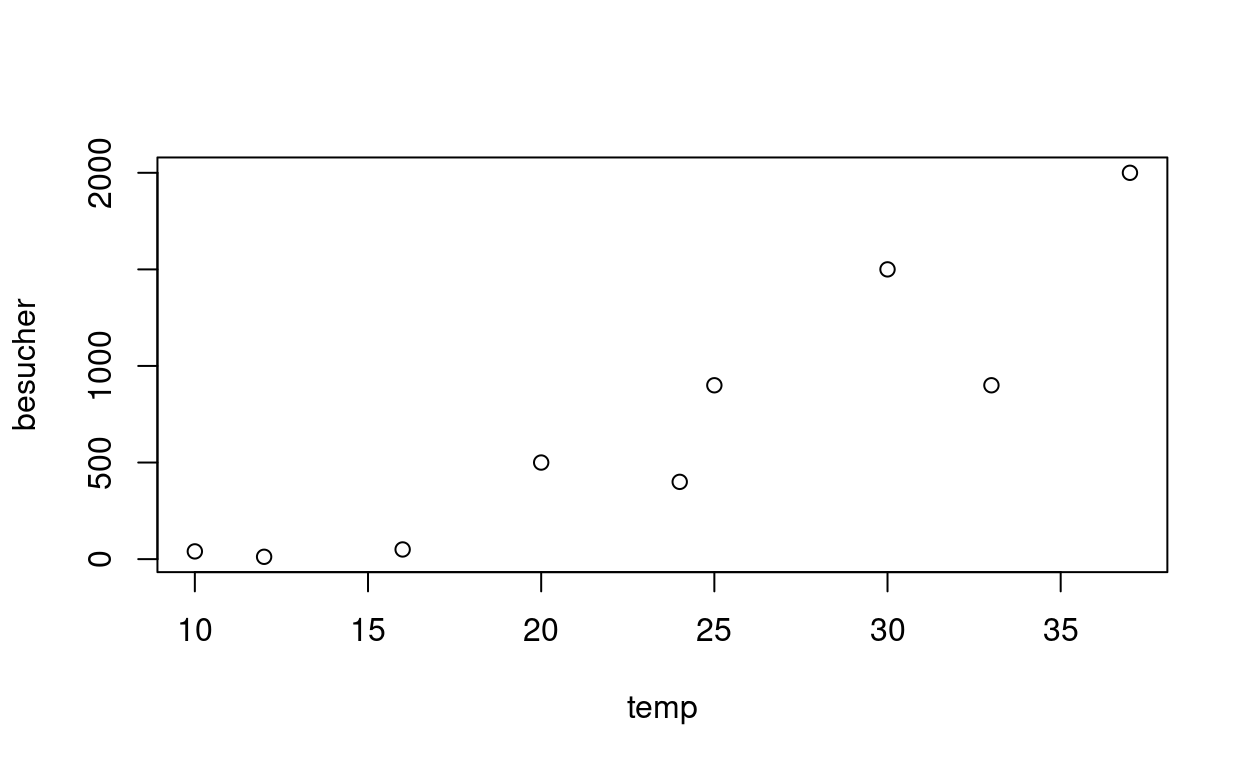
\includegraphics{solution_stat4.2s_files/figure-latex/unnamed-chunk-2-1.pdf}

\begin{Shaded}
\begin{Highlighting}[]
\CommentTok{# vieles deutet darauf hin, dass die missings (fehlende Werte) }
\CommentTok{# zufällig zustande gekommen sind (sog. MCAR); für mehr Informationen: https://uvastatlab.github.io/2019/05/01/getting-started-with-multiple-imputation-in-r/}

\CommentTok{# bester Weg wäre, die wenigen fehlenden Werte zu imputieren; }
\CommentTok{# einfachheitshalber löschen wir sie aber :)}
\NormalTok{df }\OperatorTok
\StringTok{  }\KeywordTok{drop_na}\NormalTok{()}

\CommentTok{#  sieht euch die Verteilung zwischen Mensagänger und Selbstverpfleger an}
\CommentTok{# sind nicht gleichmässig verteilt, bei der Vorhersage müssen wir das berücksichtigen}
\KeywordTok{table}\NormalTok{(df}\OperatorTok{$}\NormalTok{mensa) }
\end{Highlighting}
\end{Shaded}

\begin{verbatim}
## 
##   0   1 
## 282 786
\end{verbatim}

\begin{Shaded}
\begin{Highlighting}[]
\NormalTok{df }\OperatorTok\StringTok{ }\KeywordTok{count}\NormalTok{(mensa) }\CommentTok{# alternativ}
\end{Highlighting}
\end{Shaded}

\begin{verbatim}
## # A tibble: 2 x 2
##   mensa     n
##   <dbl> <int>
## 1     0   282
## 2     1   786
\end{verbatim}

\begin{Shaded}
\begin{Highlighting}[]
\CommentTok{# definiert das logistische Modell und wendet es auf den Datensatz an}

\NormalTok{mod0 <-}\KeywordTok{glm}\NormalTok{(mensa }\OperatorTok{~}\StringTok{ }\NormalTok{gender }\OperatorTok{+}\StringTok{ }\NormalTok{member }\OperatorTok{+}\StringTok{ }\NormalTok{age_groups }\OperatorTok{+}\StringTok{ }\NormalTok{meat }\OperatorTok{+}\StringTok{ }\NormalTok{umwelteinstellung, }
           \DataTypeTok{data =}\NormalTok{ df, }\KeywordTok{binomial}\NormalTok{(}\StringTok{"logit"}\NormalTok{))}
\KeywordTok{summary.lm}\NormalTok{(mod0) }\CommentTok{# Umwelteinstellung scheint keinen Einfluss auf die }
\end{Highlighting}
\end{Shaded}

\begin{verbatim}
## 
## Call:
## glm(formula = mensa ~ gender + member + age_groups + meat + umwelteinstellung, 
##     family = binomial("logit"), data = df)
## 
## Weighted Residuals:
##     Min      1Q  Median      3Q     Max 
## -5.6740 -0.8078  0.3712  0.5867  1.2379 
## 
## Coefficients:
##                              Estimate Std. Error t value Pr(>|t|)    
## (Intercept)                  -0.18889    0.40225  -0.470 0.638750    
## genderMann                    0.71017    0.16018   4.434 1.02e-05 ***
## memberStudent/in             -0.63072    0.29442  -2.142 0.032404 *  
## age_groups26- bis 34-jaehrig  1.09429    0.19574   5.591 2.88e-08 ***
## age_groups35- bis 49-jaehrig  1.75379    0.45968   3.815 0.000144 ***
## age_groups50- bis 64-jaehrig  2.43530    0.78923   3.086 0.002083 ** 
## meat                          0.19945    0.05055   3.945 8.49e-05 ***
## umwelteinstellung             0.19334    0.18688   1.035 0.301107    
## ---
## Signif. codes:  0 '***' 0.001 '**' 0.01 '*' 0.05 '.' 0.1 ' ' 1
## 
## Residual standard error: 1.009 on 1060 degrees of freedom
## Multiple R-squared:  0.004042,   Adjusted R-squared:  -0.002536 
## F-statistic: 0.6145 on 7 and 1060 DF,  p-value: 0.7443
\end{verbatim}

\begin{Shaded}
\begin{Highlighting}[]
\CommentTok{# Verpflegung zu haben, gegeben die Daten}

\CommentTok{# neues Modell ohne Umwelteinstellung}
\NormalTok{mod1 <-}\StringTok{ }\KeywordTok{update}\NormalTok{(mod0, }\OperatorTok{~}\NormalTok{. }\OperatorTok{-}\NormalTok{umwelteinstellung)}
\KeywordTok{summary.lm}\NormalTok{(mod1)}
\end{Highlighting}
\end{Shaded}

\begin{verbatim}
## 
## Call:
## glm(formula = mensa ~ gender + member + age_groups + meat, family = binomial("logit"), 
##     data = df)
## 
## Weighted Residuals:
##     Min      1Q  Median      3Q     Max 
## -6.0117 -0.8060  0.3584  0.6100  1.2407 
## 
## Coefficients:
##                              Estimate Std. Error t value Pr(>|t|)    
## (Intercept)                   0.03212    0.34053   0.094 0.924860    
## genderMann                    0.69697    0.15951   4.369 1.37e-05 ***
## memberStudent/in             -0.64418    0.29426  -2.189 0.028806 *  
## age_groups26- bis 34-jaehrig  1.11651    0.19458   5.738 1.25e-08 ***
## age_groups35- bis 49-jaehrig  1.77409    0.45947   3.861 0.000120 ***
## age_groups50- bis 64-jaehrig  2.44683    0.78953   3.099 0.001992 ** 
## meat                          0.18070    0.04709   3.837 0.000132 ***
## ---
## Signif. codes:  0 '***' 0.001 '**' 0.01 '*' 0.05 '.' 0.1 ' ' 1
## 
## Residual standard error: 1.01 on 1061 degrees of freedom
## Multiple R-squared:  0.003998,   Adjusted R-squared:  -0.001635 
## F-statistic: 0.7098 on 6 and 1061 DF,  p-value: 0.6418
\end{verbatim}

\begin{Shaded}
\begin{Highlighting}[]
\CommentTok{# Modeldiagnostik (wenn nicht signifikant, dann OK)}
\DecValTok{1} \OperatorTok{-}\StringTok{ }\KeywordTok{pchisq}\NormalTok{(mod1}\OperatorTok{$}\NormalTok{deviance, mod1}\OperatorTok{$}\NormalTok{df.resid) }\CommentTok{# Ok}
\end{Highlighting}
\end{Shaded}

\begin{verbatim}
## [1] 0.4509591
\end{verbatim}

\begin{Shaded}
\begin{Highlighting}[]
\CommentTok{#Modellgüte (pseudo-R²)}
\DecValTok{1} \OperatorTok{-}\StringTok{ }\NormalTok{(mod1}\OperatorTok{$}\NormalTok{dev }\OperatorTok{/}\StringTok{ }\NormalTok{mod1}\OperatorTok{$}\NormalTok{null) }\CommentTok{# eher kleines pseudo-R2}
\end{Highlighting}
\end{Shaded}

\begin{verbatim}
## [1] 0.1354244
\end{verbatim}

\begin{Shaded}
\begin{Highlighting}[]
\CommentTok{# Konfusionsmatrix vom  Datensatz}
\CommentTok{# Model Vorhersage}
\CommentTok{# hier ein anderes Beispiel: }
\NormalTok{predicted <-}\StringTok{ }\KeywordTok{predict}\NormalTok{(mod1, df, }\DataTypeTok{type =} \StringTok{"response"}\NormalTok{)}

\CommentTok{# erzeugt eine Tabelle mit den beobachteten}
\CommentTok{# Mensagänger/Selbstverpfleger und den Vorhersagen des Modells}
\NormalTok{km <-}\StringTok{ }\KeywordTok{table}\NormalTok{(predicted }\OperatorTok{>}\StringTok{ }\FloatTok{0.5}\NormalTok{, df}\OperatorTok{$}\NormalTok{mensa) }
\CommentTok{# alles was höher ist als 50% ist }
\CommentTok{# kommt in die Kategorie Mensagänger}

\CommentTok{# anpassung der namen}
\KeywordTok{dimnames}\NormalTok{(km) <-}\StringTok{ }\KeywordTok{list}\NormalTok{(}
  \KeywordTok{c}\NormalTok{(}\StringTok{"Modell Selbst"}\NormalTok{, }\StringTok{"Modell Mensa"}\NormalTok{),}
  \KeywordTok{c}\NormalTok{(}\StringTok{"Daten Selbst"}\NormalTok{, }\StringTok{"Daten Mensa"}\NormalTok{))}
\NormalTok{km}
\end{Highlighting}
\end{Shaded}

\begin{verbatim}
##               Daten Selbst Daten Mensa
## Modell Selbst           87          59
## Modell Mensa           195         727
\end{verbatim}

\begin{Shaded}
\begin{Highlighting}[]
\CommentTok{#############}
\CommentTok{### reminder: https://towardsdatascience.com/understanding-confusion-matrix-a9ad42dcfd62}
\CommentTok{#############}

\CommentTok{#TP = true positive: you predicted positive and it’s true; hier vorhersage }
\CommentTok{# mensagänger stimmt also (727)}

\CommentTok{#TN = true negative: you predicted negative and it’s true, hier vorhersage der }
\CommentTok{# selbstverpfleger stimmt (87)}

\CommentTok{#FP = false positive (fehler 1. art, auch spezifizität genannt) you predicted }
\CommentTok{# and it’s false. hier modell sagt mensagänger vorher }
\CommentTok{# (obwohl in realität selbstverpfleger) (195)}

\CommentTok{#FN = false negative (fehler 2. art, auch sensitivität genannt), }
\CommentTok{# you predicted negative and it’s false. hier modell sagt selbtverpfleger vorher }
\CommentTok{# (obwohl in realität mensagänger) (59)}


\CommentTok{# es scheint, dass das Modell häufig einen alpha Fehler zu machen, d.h. es }
\CommentTok{# das Modell weist keine hohe Spezifizität auf: konkret werden viele Mensagänger als }
\CommentTok{# Selbstverpfleger vorhergesagt resp. klassifiziert. Dafür gibt es mehere Gründe: }

\CommentTok{#1) die Kriteriumsvariable ist sehr ungleich verteilt, d.h. es gibt weniger}
\CommentTok{# Selbstverpfleger als Mensgänger im Datensatz }
 
\CommentTok{#2) nicht adäquates Modell z.B. link mit probit zeigt besserer fit}

\CommentTok{#3) Overfitting: wurde hier nicht berücksichtigt, in einem Paper/Arbeit }
\CommentTok{# müsste noch einen Validierungstest gemacht werden z.B. test-train }
\CommentTok{# Cross-Validation oder k fold Cross-Validation }

\CommentTok{# kalkuliert die Missklassifizierungsrate }
\NormalTok{mf <-}\StringTok{ }\DecValTok{1}\OperatorTok{-}\KeywordTok{sum}\NormalTok{(}\KeywordTok{diag}\NormalTok{(km)}\OperatorTok{/}\KeywordTok{sum}\NormalTok{(km)) }\CommentTok{# ist mit knapp 23 %  eher hoch}
\NormalTok{mf}
\end{Highlighting}
\end{Shaded}

\begin{verbatim}
## [1] 0.2378277
\end{verbatim}

\begin{Shaded}
\begin{Highlighting}[]
\CommentTok{# kleiner exkurs: https://www.ncbi.nlm.nih.gov/pmc/articles/PMC2636062/}
\CommentTok{# col wise proportion, da diese die "realität" ist}
\NormalTok{km_prop <-}\StringTok{ }\KeywordTok{prop.table}\NormalTok{(km,}\DecValTok{2}\NormalTok{)}


\CommentTok{# specificity = a / (a+c) => ability of a test to correctly }
\CommentTok{# classify an individual as disease-free is called the test′s specificity}
\NormalTok{spec =}\StringTok{ }\NormalTok{km_prop[}\DecValTok{1}\NormalTok{] }\OperatorTok{/}\StringTok{ }\NormalTok{(km_prop[}\DecValTok{1}\NormalTok{] }\OperatorTok{+}\StringTok{ }\NormalTok{km_prop[}\DecValTok{2}\NormalTok{])}
\NormalTok{spec}
\end{Highlighting}
\end{Shaded}

\begin{verbatim}
## [1] 0.3085106
\end{verbatim}

\begin{Shaded}
\begin{Highlighting}[]
\CommentTok{# sensitivity = d / (b+d) => Sensitivity is the ability of a }
\CommentTok{# test to correctly classify an individual as ′diseased′}
\NormalTok{sens =}\StringTok{ }\NormalTok{km_prop[}\DecValTok{4}\NormalTok{] }\OperatorTok{/}\StringTok{ }\NormalTok{(km_prop[}\DecValTok{3}\NormalTok{] }\OperatorTok{+}\StringTok{ }\NormalTok{km_prop[}\DecValTok{4}\NormalTok{])}
\NormalTok{sens}
\end{Highlighting}
\end{Shaded}

\begin{verbatim}
## [1] 0.9249364
\end{verbatim}

\begin{center}\rule{0.5\linewidth}{0.5pt}\end{center}

\textbf{Methode}

In der Aufgabe war es das Ziel zu schauen, ob wir einen potenziellen
Besuch eines Mensagasts vorhersagen können und zwar in Abhängigkeit von
den sozioökonimischen Variablen, wahrgenommene Fleischkonsum und der
Umwelteinstellung. Die Kriteriumsvariable ``Mensa'' weist eine binäre
Verteilung auf: Deshalb rechnen wir eine multiple logistische Regression
mit den Prädiktoren ``Alter'', ``Geschlecht'',
``Hochschulzugehörigkeit'', ``Fleischkonsum'' und "Umwelteinstellung.
Mehr Informatinen zu den logistischen Regressinen findet ihr im Buch von
Crawley (2015) oder auch im Buch von
\href{http://faculty.marshall.usc.edu/gareth-james/ISL/ISLR\%20Seventh\%20Printing.pdf}{Gareth
(2016)}, Kapitel 4.3; passendes Video
\href{https://www.youtube.com/watch?v=31Q5FGRnxt4\&list=PL5-da3qGB5IC4vaDba5ClatUmFppXLAhE\&index=2}{hier}.

\begin{center}\rule{0.5\linewidth}{0.5pt}\end{center}

\textbf{Ergebnisse}

\begin{longtable}[]{@{}lrr@{}}
\toprule
& Daten Selbst & Daten Mensa\tabularnewline
\midrule
\endhead
Modell Selbst & 87 & 59\tabularnewline
Modell Mensa & 195 & 727\tabularnewline
\bottomrule
\end{longtable}

Der Output des logistischen Models mit der Linkfunktin ``logit'' sagt
und, dass das Modell nicht gut zu den Daten passt, d.h. mit dem Modell
(gegeben die Daten) können wir nur schlecht vorhersagen, ob eine Person
zukünftig sich in der Mensa verpflegt oder ihr Mittagessen selber
mitnimmt. Hinweise dafür geben das kleine pseudo-R2 (14\%) als auch die
hohe Missklassifizierungsrate (24\%): bei genauerer Betrachtung fällt
auf, dass das Modell häufig einen alpha-Fehler begeht, d.h. unser Modell
sagt zu viele Mensagänger vorher, obwohl diese in Realität
Selbstverpfleger sind. Es gibt verschiedene Gründe für diesen schlechten
Modelfit:

\begin{itemize}
\tightlist
\item
  die Kriteriumsvariable ist sehr ungleich verteilt, d.h. es gibt
  weniger Selbstverpfleger als Mensgänger im Datensatz (26\% vs.~74\%)
\item
  die Prädiktorvariablen sind alle entweder kategorial oder ordinal:
  dies kann dazu führen, dass das Model keinen guten fit zu den Daten
  erzielt
\end{itemize}

\textbf{Fazit}: Es sollte nach einem weiteren adäquateren Modell gesucht
werden: insbesondere ein Modell, welches einen mit ordinalen
Prädiktorvariablen umgehen kann:

\begin{itemize}
\tightlist
\item
  eine bessere Link-Funktion für das GLM suchen z.B. probit
\item
  \href{https://stats.stackexchange.com/questions/195246/how-to-handle-ordinal-categorical-variable-as-independent-variable}{polynomiale
  Kontraste}
\item
  Smooth Splines
  \href{https://www.frontiersin.org/articles/10.3389/fams.2017.00015/full}{hier}
\end{itemize}

\end{document}
